\documentclass[english,serif,mathserif,xcolor=pdftex,dvipsnames,table]{beamer}
\usetheme[informal]{gc3}
\usepackage{gc3}

\title[Introduction]{%
  Do not reinvent the wheel:
  \\
  A survey of useful Python packages
}
\author[GC3]{%
  GC3: Grid Computing Competence Center, \\
  University of Zurich
}
\date{Mar.~19--20, 2014}

\begin{document}

% title frame
\maketitle

\begin{frame}
  \frametitle{There is more to Python than this\ldots}

  The time and scope of this course is rather limited.

  \+
  Here is an (incomplete) list of Python features that you might
  want to look up as you become more experienced in the language:
  % XXX: mettere un link per ciascuna di queste!
  \begin{itemize}
  \item
    \href{http://docs.python.org/2/tutorial/classes.html\#generators}{Generators}
    and
    \href{http://docs.python.org/2/tutorial/classes.html\#iterators}{Iterators}
  \item \href{http://www.artima.com/weblogs/viewpost.jsp?thread=240808}{Decorators}
  \item Class-level attributes, \href{http://stackoverflow.com/a/12179752/1808780}{classmethods, staticmethods}
  \item Properties and accessors
  \item \href{http://stackoverflow.com/a/6581949/459543}{Metaclasses}
  \end{itemize}
\end{frame}


\begin{frame}
  \frametitle{matplotlib: publication quality plotting library}

  \href{http://matplotlib.org/}{matplotlib} ``is a python 2D plotting
  library which produces publication quality figures in a variety of
  hardcopy formats and interactive environments across
  platforms. matplotlib can be used in python scripts, the python and
  ipython shell (ala MATLAB® or Mathematica®), web application
  servers, and six graphical user interface toolkits.''
\end{frame}


\begin{frame}
  \frametitle{NumPy: linear algebra package}

  \href{http://www.numpy.org/}{NumPy} is a package for linear algebra
  and advanced mathematics in Python.

  \+ It provides a \emph{fast} implementation of multidimensional
  numerical arrays (C/FORTRAN like), vectors, matrices, tensors and
  operations on them.

  \+ \emph{Use it if:} you long for MATLAB core features.

  \begin{seealso}
    \url{http://www.numpy.org/}
  \end{seealso}
\end{frame}


\begin{frame}
  \frametitle{SciPy: a toolbox for numerics}

  ``\href{http://www.scipy.org}{SciPy} is open-source software for
  mathematics, science, and engineering. \emph{[\ldots]} The SciPy
  library provides many user-friendly and efficient numerical routines
  such as routines for numerical integration and optimization.''

  \+ One of its main aim is to provide a reimplementation of the
  MATLAB toolboxes.

  \+ \emph{Use it if:} you long for MATLAB toolbox features.

  \begin{seealso}
    \url{http://www.scipy.org/}
  \end{seealso}
\end{frame}


\begin{frame}
  \frametitle{Pandas: doing statistics in Python}

  \href{http://pandas.pydata.org/}{Pandas} is a Python data analysis
  library, that provides optimized routines for analyzing 2D, 3D, 4D
  data.

  \+ ``Pandas \emph{[\ldots]} enables you to carry out your entire
  data analysis workflow in Python without having to switch to a more
  domain specific language like R.''

  \+ \emph{Use it if:} you need features from \emph{R}, \texttt{plyr},
  \texttt{reshape2}.
\end{frame}


\begin{frame}
  \frametitle{NLTK: Natural Language Processing}

  \href{http://nltk.org/}{NLTK} \emph{(Natural Language ToolKit)} ``is
  a leading platform for building Python programs to work with human
  language data. It provides easy-to-use interfaces to over 50 corpora
  and lexical resources such as WordNet, along with a suite of text
  processing libraries for classification, tokenization, stemming,
  tagging, parsing, and semantic reasoning.''

  \+ This is considered one of the leading natural language parsing
  libraries, not just for Python.
\end{frame}


\begin{frame}
  \frametitle{SQLAlchemy: portable access to databases}

  \href{http://www.sqlalchemy.org/}{SQLAlchemy} is a Python library
  that provides portable and powerful access to SQL databases, with a
  natural Python syntax.

  \+ \href{http://www.sqlalchemy.org/}{SQLAlchemy} frees you and your
  code from knowing SQL syntax and the annoying little differences
  among DBs: the same code would run witl SQLite, MySQL, PostgreSQL,
  MS-SQL, Oracle, etc.
\end{frame}

\begin{frame}
  \frametitle{PyCLI: writing command line applications}

  The \href{https://pypi.python.org/pypi/pyCLI}{cli package} is a
  framework for making simple, correct command line applications in
  Python.

  \+
  With cli, you can quickly add standard command line parsing;
  logging; unit and functional testing; and profiling to your CLI
  apps.
\end{frame}


\begin{frame}
  \frametitle{sh: a module to easily call external programs}

  \href{http://amoffat.github.com/sh/}{sh} allows you to call any
  program as if it were a function.

  \+

  It makes very easy to write \texttt{bash}-like scripts in Python.

  \+

  It supports optional arguments, pipes, I/O redirection, with a
  trivial syntax.
\end{frame}

\begin{frame}
  \frametitle{virtualenv: a tool to create isolated Python environments}

  \href{https://pypi.python.org/pypi/virtualenv}{virtualenv} is a very
  useful tool to create, as \textit{regular user}, multiple,
  indepentend environments and install a variety of Python packages in
  them.

  \begin{itemize}
  \item environments are created and deleted easily (\texttt{rm -rf <directory>}
  \item you can install the latest version of a package using
    \texttt{pip install <package>}
  \item you can have multiple, incompatible environments installed on
    the machine and just use them one at a time.
  \end{itemize}
\end{frame}


\begin{frame}
  \frametitle{Want more? Look into PyPI}

  \href{http://pypi.python.org}{PyPI} is \emph{the} index of Python software packages.

  \+ It currently indexes 28948 packages, so the choice is really vast.

  \+ Almost all packages can be installed with a single command by
  running \href{https://pypi.python.org/pypi/pip}{\texttt{pip install
    \emph{packagename}}}.

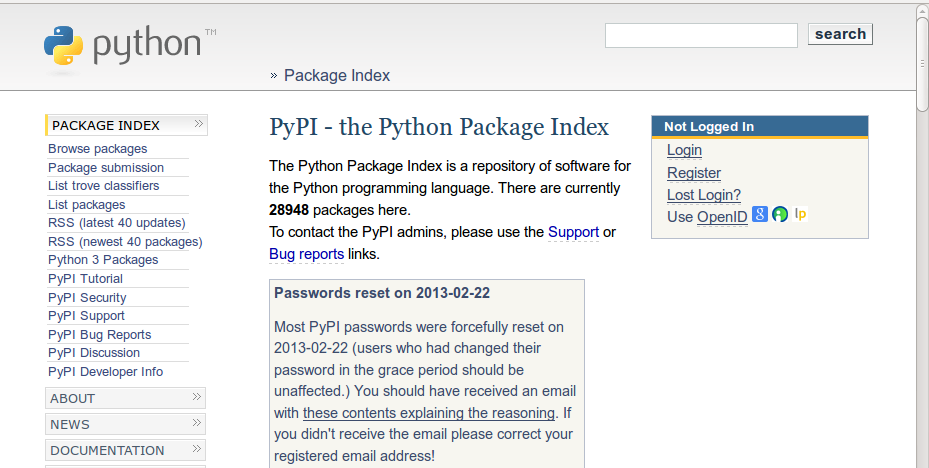
\includegraphics[width=1\textwidth]{fig/pypi_screenshot.png}
\end{frame}

\end{document}
